\documentclass[journal]{IEEETran}
\usepackage{bm}
\usepackage{times}
\usepackage{graphicx}
\usepackage{psfrag}
\usepackage{epsfig}
\usepackage{algorithm}
\usepackage{algorithmic}
%\usepackage{algpseudocode}
\usepackage{multicol}
\usepackage{multirow}
\usepackage{setspace}
%\usepackage{subfigure}
\usepackage{cite}
\usepackage{array}
\usepackage{amssymb}
\usepackage[cmex10]{amsmath}
\interdisplaylinepenalty=2500
\usepackage{mdwmath}
\usepackage{mdwtab}
\usepackage[tight,footnotesize]{subfigure}
%\usepackage{fixltx2e}
\usepackage{mdwlist}
\usepackage{epstopdf}

\usepackage{caption, color}
%\usepackage{slashbox}
\usepackage{yhmath}
%\numberwithin{equation}{section}
%\usepackage{footnpag}
\twocolumn
\singlespacing

\newtheorem{thm}{Theorem}
\newtheorem{lemma}[thm]{Lemma}
\newtheorem{property}[thm]{Property}



\begin{document}


\title{Joint Power and Resource Allocation for Non-Uniform Topologies in Heterogeneous Networks}



\author{\IEEEauthorblockN{Shangzhang~Zou, Nan Liu, Zhiwen Pan and Xiaohu You}\\
\IEEEauthorblockA{National Mobile Communications Research Laboratory, Southeast University, Nanjing, China\\
Email: zou.szhang@gmail.com, \{nanliu, pzw, xhyu\}@seu.edu.cn\\}
\thanks{
This work is partially
supported by the National Basic Research Program of China
(973 Program 2012CB316004), the National Natural Science Foundation of China
under Grants $61201170$, $61271208$ and $61221002$ and Qing Lan Project.}
}

\maketitle

\begin{abstract}
 Enhanced Inter Cell Interference Coordination (eICIC) for co-channel deployments of pico cells in a macro cell layout is studies. In particular, we consider a scenario where only some macro cells have picos deployed, while other macro cells have no picos. The interference caused by a macro to pico cells can be mitigated by having the macro mute some of its subframes. We consider a joint problem of power and resource allocation. The goal is to maximize the PF utility, and solve this problem. The simulation results demonstrated that our proposed algorithms improve the user throughput in both the macros with picos and without picos.
\end{abstract}
\section {Introduction}\label{Introduction}

\IEEEPARstart{W}{ireless} data traffic has vastly grown in recent years. The traditional cellular network can not meet the needs of high-growth data. Addressing the rapid growth in wireless data need to improve the spectrum efficient. An important method to making the radio spectrum efficient is LTE heterogeneous networks (LTE HetNets)\cite{OverviewHetNets}. In a HetNet architecture, in addition to usual macrocells, the low power nodes can also deployed in the network. Low power nodes in LTE HetNets is general refer to femtocells and picocells. Such HetNets enable a more flexible, targeted, and economical deployment of infrastructure. Low power nodes typically share the same frequency band as macrocells, the performance of low power nodes could be severely affect by high power macro node. In order to solve the cross-tier interference problem, LTE standards support a time domain pattern for muting transmissions of the macro\cite{eICICIntroduction}, which is also called enhanced Intersect Interference Coordination (eICIC). In eICIC, the interference caused by a macro to pico cells can be mitigated by having the macro mute some of its subframes. These are known as \textit{Almost Blank Sub-frames} (ZP-ABS) which stop data transmission during subframes or \textit{Low Power Sub-frames} (LP-ABS) which simply reduce the transmission power during subframes.

\begin{figure}[htpb]
\centering
\includegraphics[width=.5\textwidth]{macroAndPico.pdf}
\caption{Typical HetNet architecture with a macro cell and a pico cell, each cell regard as two logic cell.}
\label{F_macroAndPico}
\end{figure}

LP-ABS can decrease the influence of ABSs on the throughput of macro UEs because the macro UE can transmit data on both ABS and non-ABS. On the other hand, using ABS and non-ABS by macro UEs causes the throughput of UEs in pico to decrease because of interference from macro on the ABSs. The proportion of muted sub-frames needs to be carefully chosen. Note that the proper proportion of muted sub-frames is related to the number of users assigned to the picos and the number of users assigned to macros. The more users assigned to macros, the greater the cost of macro for muting. In LP-ABS, both macro and pico can scheduling users in ABS sub-frames, so determine the users whom it should allocate the ABS resources and whom it should allocated the non-ABS resources is also an important issue. The other important parameter which is taken into account in LP-ABS scheme is the level of transmission power reduction. When the transmission power just reduce a little the macro UE?¡¥s throughput is not improved significantly because the received signal quality of macro UE on ABSs is poor. On the other hand, if the reduction in the power level is very low, the throughput of UEs located in range expanded area decreases compared to ZP-ABS because these UEs still suffer the interference from the macro eNBs on ABSs. Therefore, there are four factors associated with interference management problem as following (a) which users should be assigned to macro cells and pico cells, each cell also has to decide (b) which users should receive resource from ABS or non-ABS, (c) what the muting proportion should be, and (d) the level of transmission power macro reduction.

For scenarios with the same number of picos in all macros, it can using the same muting pattern at all macros\cite{AlgorithmEicic} and using LP-ABS only to solve problem \cite{JointABSPower}. However, it is not worth using eCIC of cases where only a few picos are deployed in some macros. A realistic non-uniform HetNets is been introduced in \cite{NonUniformTopologies}, the results show that coordinate use of ZP-ABS and LP-ABS can reach high system performance in this kind of topologies. But how to coordinate macro muting patterns is not mentioned. In this paper show how to solve this problem.

The main contributions are summarized as follows. (a) We formulate the optimization problem of all the above aspects. The goal is to maximize the sum logarithmic utility of all users to maintain network-wide proportional fairness. (b) We decouple the joint problem into four subproblems and solve each of them in an alternating manner.

The structure of this paper is as follows: In Section \ref{Section 2}, we presents the system model and formulates the joint optimization problem. In Section \ref{Section 3}, we studies the four components of the optimization problem, and solving each of them. Numerical evaluation is shown in Section \ref{Section 4}. Finally, Section \ref{conclusion} summarizes this paper.


\section{System  Model and Problem Formulation}\label{Section 2}
  In this section, we consider the downlink transmission in eICIC HetNet with macro base stations configured with low power ABSs and formulate a PF utility optimization problem.

\subsection{System Model}\label{System model}
Consider a HetNet consisting of $N$ UEs, $M$ macros configured with LP-ABS and $P$ picos. We denote $\mathcal{U}$ as the set of all users.
%Each cell has a unit resource that it can allocate amongst the users.
We assume a repeating ABS pattern of frames configured at the macros, and synchronous ABS configuration is considered, i.e. all macro base stations configure LP-ABS in the same set of sub-frames. The proportion of the sub-frames used as LP-ABS for all the macros is taken to be $\beta$. Unlike zero-ABS where macros only transmit in nABS subframes, in LP-ABS macros can also transmit in ABS subframes, albeit with a low power. We can visualize each macro or pico cell as consisting of two sub-cells, one which is active only during ABS and can allocate a fraction $\beta$ of the cell's total resource blocks, and the other which is active only during nABS and can allocate a fraction $(1 - \beta)$ of the cell's total resource blocks. Thus, we can assume that there are $2(M + P)$ cells in the networks. Denote the set of macro sub-cells that is active only during ABS (nABS) as $\mathcal{M}_{ABS}$ ($\mathcal{M}_{nABS}$), and the set of pico sub-cells that is active only during ABS (nABS) as $\mathcal{P}_{ABS}$ ($\mathcal{P}_{nABS}$).
%For example, in Fig.\ref{F_macroAndPico}, MABS-UE, MnABS-UE, PABS-UE and PnABS-UE are associated to $\mathcal{M}_{ABS}$, $\mathcal{M}_{nABS}$, $\mathcal{P}_{ABS}$ and $\mathcal{P}_{nABS}$, respectively.
 %We consider following rule: the UEs associated to $\mathcal{M}_{ABS}$ or $\mathcal{P}_{ABS}$ can be scheduled only during ABS, while the UEs associated to $\mathcal{M}_{nABS}$ or $\mathcal{P}_{nABS}$ can be scheduled only during nABS.
 %We assume that all eNBs have full buffers.

 The four subsets of cells create four different downlink interference patterns. The SINR of UE-$u$ associated with macro sub-cell $b$ can be written as:

\begin{align}\label{SINR1}
&{SINR}_{ub}=\nonumber \\
&\left\{
\begin{matrix}
{\frac{P_bG_{ub}}{{\sum\nolimits_{k \in \mathcal{M}_{ABS},k \ne b} {{P_k}{G_{uk}} + \sum\nolimits_{k \in \mathcal{P}_{ABS}} {{P^{P}}{G_{uk}} + {N_0}} } }},b\in \mathcal{M}_{ABS}}\\
{\frac{P^{M}G_{ub}}{{\sum\nolimits_{k \in {\mathcal{M}_{nABS}},k \ne b} {{P^{M}}{G_{uk}} + \sum\nolimits_{k \in {\mathcal{P}_{nABS}}} {{P^{P}}{G_{uk}} + {N_0}} } }},b\in \mathcal {M}_{nABS}}\\
\end{matrix}
\right.
\end{align}
where $P_b$ is the transmission power of macro sub-cell $b$, $b \in \mathcal{M}_{ABS}$, $P^M$ is the transmission power of all macro cells on the normal subframes, $P^P$  is the transmission power of all pico cells on all subframes, $G_{ub}$ is the channel gain between sub-cell $b$ and UE $u$, and the two subcells have the same channel gain if they are split from the same cell, and $N_0$ is the noise power. On the other hand, the SINR expression of UE $u$ associated with pico sub-cell $b$ is:

\begin{align}\label{SINR2}
&{SINR}_{ub}=\nonumber \\
&\left\{
\begin{matrix}
{\frac{P^{P}G_{ub}}{{\sum\nolimits_{k \in \mathcal{M}_{ABS}}{{P_k}{G_{uk}} + \sum\nolimits_{k \in \mathcal{P}_{ABS},k \ne b} {{P^{P}}{G_{uk}} + {N_0}} } }},b\in \mathcal{P}_{ABS}}\\
{\frac{P^{P}G_{ub}}{{\sum\nolimits_{k \in {\mathcal{M}_{nABS}}}{{P^{M}}{G_{uk}} + \sum\nolimits_{k \in {\mathcal{P}_{nABS}},k \ne b} {{P^{P}}{G_{uk}} + {N_0}} } }},b\in \mathcal {P}_{nABS}}\\
\end{matrix}
\right.
\end{align}

We use the Shannon capacity formula to obtain $R_{ub}$ which denotes the the expected data rate of UE $u$ associated with sub-cell $b$:
\begin{align}\label{Rate}
R_{ub} = B\log_2(1+SINR_{ub})
\end{align}
where $B$ represents the total bandwidth of the system. 

\subsection{Problem Statement}\label{Problem Statement}
The object of the paper is system throughput maximization with proportional fairness. We use indicators $\{x_{ub}\}$ to represent user-cell association, i.e., $x_{ub} = 1$ when user $u$ is associated with cell $b$, and $x_{ub} = 0$ otherwise. We assume that a UE can only associate with one logical cell, and thus the UE association constraint is:
\begin{align}
\sum_{b \in \mathcal{B}}x_{ub} = 1,~~ \forall u \in \mathcal{U}
\end{align}
where $\mathcal{B} = \mathcal{M}_{ABS} \cup \mathcal{M}_{nABS} \cup \mathcal{P}_{ABS} \cup \mathcal{P}_{nABS}$ is the collection of all logical cell. This is in accordance with \cite{OptimalMutingAndLoad}, which showed that when maximizing the proportional fairness utility in eICIC, some UEs are scheduled to transmit only in the ABS subframes and the remaining UEs are scheduled to transmit only in the non-ABS subframes. 

Denote $\{y_{ub}\}$ as the proportion of resource allocated to UE $u$ by cell $b$. A cell can only allocate its resource to the UEs associated with it. Hence we have the resource allocation constraints:
\begin{subequations}
\begin{align}
&\sum_{u \in \mathcal{U}}y_{ub} = (1 - \beta),& b \in \mathcal{B}_{nABS}\\
&\sum_{u \in \mathcal{U}}y_{ub} = \beta,& b \in \mathcal{B}_{ABS}\\
&0 \leq y_{ub} \leq x_{ub}, &\forall u \in \mathcal{U}, \forall b \in \mathcal{B}
\end{align}
\end{subequations}
where $\mathcal{B}_{nABS} = \mathcal{M}_{nABS} \cup \mathcal{P}_{nABS}$ and $\mathcal{B}_{ABS} = \mathcal{M}_{ABS} \cup \mathcal{P}_{ABS}$. The transmission power of LP-ABS in macro cells can not exceed the maximum transmit power $P^M$. Hence we have the $\{P_b\}$ constraints:
\begin{align}\label{constraint p}
0 \leq P_b \leq P^M,~~~~b \in \mathcal{M}_{ABS}
\end{align}

The optimization objective we choose is the proportional fairness utility. It is well known that the proportional fairness objective strikes a good balance between system throughput and UE-throughput fairness\cite{JainFairness}. Hence the considered problem can be formulated as:
\begin{align}\label{optimization obj}
&\max_{\{\beta,x_{ub},y_{ub},P_b\}} \sum_{b \in \mathcal{B}} \sum_{u \in \mathcal{U}} x_{ub} \log (y_{ub}R_{ub})\\
&~~~~~~s.t.~~~~(\ref{SINR1}) - (\ref{constraint p}) \notag
\end{align}

\section{Problem solutions}\label{Section 3}
The optimization problem is NP-hard even with a single macro and a single pico . We can prove the above problem is a NP-hard problem, we reduce the infinite number of the possible transmit power of each cell in problem into a fixed value, $0$ for example, and formulate a new problem we called reduced problem. Since the reduced problem is just a special case of the original problem, if the reduced problem can be proved NP-hard, the original problem is also NP-hard.
The reduced problem is proved NP-hard \cite{AlgorithmEicic}, so our problem is a NP-hard problem. We develop an suboptimal solution to find optimal UE association, ABS allocation and transmit power in LP-ABS. At each iteration of the method, a singal block of variables is optimized and remaining variables are fixed. We decompose the optimization variables into four blocks: $\{x_{ub}, y_{ub}\}$, $\beta$ and $\{P_b\}$ which relate with the three sub-problems respectively: the UE association and the resource allocation, the ABS allocation and the transmit power in LP-ABS.

\subsection{Optimizing $\{ x_{ub}, y_{ub} \}$ for given $\beta$ and $\{ P_b \}$}\label{optimizing y}
For determining the resource allocation $\{x_{ub},y_{ub}\}$, we assume that the other optimization variables, i.e., $\beta$ and $\{ P_b \}$, are given and fixed. 

First, for a fixed $\{x_{ub}\}$, we find the optimal $\{y_{ub}\}$: the optimization problem can be decomposed into two sets of subproblems as follows:
\begin{align} \label{optimizing y 1}
&\forall b \in \mathcal{B}_{ABS} : \nonumber \\
& \max_{\{y_{ub}\}} \sum_{u \in \mathcal{U}_b} \log (y_{ub}R_{ub})\\
& s.t.\sum_{u \in \mathcal{U}_b} y_{ub} = (1 - \beta)\notag \\
& 0 \leq y_{ub} \leq 1,~~\forall u \in \mathcal{U}_b \notag
\end{align}

\begin{align} \label{optimizing y 2}
&\forall b \in \mathcal{B}_{nABS} : \nonumber \\
& \max_{\{y_{ub}\}} \sum_{u \in \mathcal{U}_b} \log (y_{ub}R_{ub})\\
& s.t.\sum_{u \in \mathcal{U}_b} y_{ub} = \beta \notag \\
& 0 \leq y_{ub} \leq 1,~~\forall u \in \mathcal{U}_b \notag
\end{align}
where $\mathcal{U}_b$ is the set of UEs associated to cell $b$. We can see that the above subproblems of (\ref{optimizing y 1}) and (\ref{optimizing y 2}) are convex and mutually independent, and we can use the proportional fairness (PF) scheduling algorithm \cite{PFSchedulingAlgorithm} to solve the problems, and the optimal resource allocation is \cite{PFSchedulingAlgorithm}
\begin{align}\label{best y}
  y_{ub} = \left\{
\begin{matrix}
{ \frac{1 - \beta}{ \sum_{k \in \mathcal{U}}{x_{kb}}},~~\forall b \in \mathcal{B}_{nABS} } \\
{ \frac{\beta}{ \sum_{k \in \mathcal{U}}{x_{kb}}},~~\forall b \in \mathcal{B}_{ABS} }
\end{matrix}
\right.
\end{align}
Equation (\ref{best y}) means that the optimal resource allocation is equal allocation among all UEs associated to cell $b$.

Next, we find the optimal UE association $\{x_{ub}\}$. Plugging the optimal $y_{ub}$ found in (\ref{best y}) into (\ref{optimization obj}), the UE association problem can be written as:
\begin{align}\label{optimizing x obj}
  \max_{\{x_{ub}\}} &\sum_{b \in \mathcal{B}} \sum_{u \in \mathcal{U}} x_{ub} \log(\frac{\overline{R}_{ub}}{ \sum_{k \in \mathcal{U}} x_{kb}}) \\
  s.t.~~&\sum_{b \in \mathcal{B}} x_{ub} = 1,\forall u \in \mathcal{U} \notag\\
  &x_{ub} \in \{ 0,1 \},\forall u \in \mathcal{U}, \forall b \in \mathcal{B} \notag
\end{align}
where
\begin{align*}
\overline{R}_{ub} = \left\{
  \begin{matrix}
    (1-\beta)R_{ub},&\forall b \in \mathcal{B}_{nABS} \\
    \beta R_{ub},&\forall b \in \mathcal{B}_{ABS} \\
  \end{matrix}
  \right.
\end{align*}
The problem (\ref{optimizing x obj}) is combinatorial due to the binary variable $x_{ub}$. The complexity of the brute force algorithm is $\Theta((2M + 2P)^N)$, where $(2M + 2P)$ and $N$ denote the number of logical cells and number of users, respectively. Multilayer user association \cite{UserAssociation} and issue considered in this section is very similar, except that \cite{UserAssociation} does not use ABS to eliminate the interference in pico cells. But we also can use his methods to solve our problems. Because in our paper we treat each cell as two virtual cells, when the other parameters fixed the user from a different virtual cells to obtain a desired rate is determined. This feature makes the two of the problem is the same, the different is our problem need to associate users between $(2M + 2P)$ cells. Here we only present part of the algorithm.

First, relax the binary constraint on ${x_{ub}}$ which mean to allow users to be associated to more than one cells to make problem convex. Then, decouple the dual problem of into two sub-problems $f_x(\mu)$ and $g_K(\mu)$,
\begin{align}\label{dualProblem}
  \bm{D}:~~\min_\mu D(\mu) = f_x(\mu) + g_K(\mu),
\end{align}
where
\begin{align} \label{optimizing x UE}
  &f(\mu) = \left\{
  \begin{matrix}
  \max\limits_{\bm{x}} &\sum\limits_{b \in \mathcal{B}} \sum\limits_{u \in \mathcal{U}} x_{ub}(\log(\overline{R}_{ub}) - \mu_b) \\
  s.t. &\sum\limits_{b \in \mathcal{B}} x_{ub} = 1 \\
   &0 \leq x_{ub} \leq 1
  \end{matrix}
  \right.
\end{align}
\begin{align}\label{optimizing x BS}
  &g(\mu) = \max \sum\limits_{b \in \mathcal{B}} K_b(\mu_b - \log(K_b))
\end{align}
where $\mu_b$ is Lagrange multiplier. which be solved separately on users' side and cells' side respectively. Optimizing $f(\mu)$ should satisfies the follows
\begin{align}\label{optimizingX1}
  b^* = \arg \max_b (\log(R_{ub}) - \mu_b(t))
\end{align}
means UE-$u$ associate to cell-$b^*$, $t$ represent times of teration. To obtain the maximize problem $g(\mu)$ we set its gradient to be 0, i.e.
\begin{align}\label{optimizingX2}
 K_b(t) = e^{(\mu_b(t) - 1)}
\end{align}
then the value of the Lagrange multiplier is updated by
\begin{align}\label{optimizingX3}
\mu_b(t+1) = \mu_b(t) - \delta(t)\cdot(K_b(t) - \sum\limits_{u \in \mathcal{U}} x_{ub}(t))
\end{align}
where $\delta(t) > 0$ is a dynamically chosen stepsize sequence, see Appendix for detail. Repeat step (\ref{optimizingX1}), (\ref{optimizingX2}) and (\ref{optimizingX3}) until $D(\mu)$ convergence.

\subsection{Optimizing $\beta$ for Given $\{ y_{ub}, x_{ub} \}$ and $\{ P_b \}$}\label{optimizing beta}
In this subsection we discuss the ABS allocation. The other optimization variables are fixed, the joint problem can be rewritten as:
\begin{align}
  \max_{\beta} \sum_{b \in \mathcal{B}_{nABS}} \sum_{u \in \mathcal{U}_b} & \log(\frac{ (1 - \beta)R_{ub} }{ \sum\limits_{u \in \mathcal{U}_b} x_{ub}}) \notag\\
  &+ \sum_{b \in \mathcal{B}_{ABS}} \sum_{u \in \mathcal{U}_b} \log(\frac{ \beta R_{ub} }{ \sum\limits_{u \in \mathcal{U}_b} x_{ub}}) \\
  &s.t.~~0 < \beta < 1. \notag
\end{align}

The above-mentioned formulation is convex, and only one variable. We can let the gradient of the objective function equal zero.so the optimal ABS configuration is
\begin{align}
    \beta^\star = \frac{\sum\limits_{b \in \mathcal{B}_{ABS}} \sum\limits_{u \in \mathcal{U}_b} 1}{N}
\end{align}
Where $N$ is the sum num of UEs.In other words, the optimal ABS rate tracks the fractional sum of the UEs in the ABS
. This is because the ABS resources are allocated to the UEs associated within the $\mathcal{B}_{nABS}$.

\subsection{Optimizing $\{ P_b \}$ for Given $\{ y_{ub}, x_{ub} \}$ and $\beta$ }\label{optimizing p}
In this subsection, we discuss the transition power of macro cell in ABS sub-frames, while other optimization variables are fixed. We assume each macro cell can set different transition power in ABS sub-frames, The optimization problem can be rewritten as:
\begin{align} \label{optimizing p obj}
  \max_{\bm{P}} \sum_{b \in \mathcal{B}_{nABS}} \sum_{u \in \mathcal{U}_b} & \log(\frac{ (1 - \beta)R_{ub} }{ \sum\limits_{u \in \mathcal{U}_b} x_{ub}}) \notag\\
  &+ \sum_{b \in \mathcal{B}_{ABS}} \sum_{u \in \mathcal{U}_b} \log(\frac{ \beta R_{ub} }{ \sum\limits_{u \in \mathcal{U}_b} x_{ub}}) \\
  s.t.~~& 0 < P_b < P^{M}, b \in \mathcal{M}_{ABS} \notag
\end{align}
Where $\bm{P} = \{P_b\}, b \in \mathcal{M}_{ABS}$, donate the transition power of macro cell in ABS sub-frames, the transition power of macro cell in ABS sub-frames can choose between zero and max transition power. Considering (\ref{SINR1}), (\ref{SINR2}) and (\ref{Rate}), only ${R_{ub}}$ where $b \in \mathcal{B}_{ABS}$ are associated to $\bm{P}$, we just need to solving the part of optimization problem while the part of the rest is constant. Therefore, (\ref{optimizing p obj}) can be rewritten as:
\begin{align} \label{optimizing p g}
 \max_{\bm{P}}~~g(\bm{P}) = \sum_{b \in \mathcal{B}_{ABS}} \sum_{u \in \mathcal{U}_b} \log(\frac{ \beta R_{ub} }{ \sum\limits_{u \in \mathcal{U}_b} x_{ub}}) \\
 s.t.~~0 < P_b < P^{M}, b \in \mathcal{M}_{ABS} \notag
\end{align}
when other optimization variables are fixed, means $\beta$ and $\sum\limits_{u \in \mathcal{U}_b} x_{ub}$ are fixed and no effects to utility function solving. Therefore, (\ref{optimizing p g}) is equivalent to
\begin{align} \label{optimizing p f}
 \max_{\bm{P}}~~f(\bm{P}) = \sum_{b \in \mathcal{B}_{ABS}} \sum_{u \in \mathcal{U}_b} \log(R_{ub}) \\
 s.t.~~0 < P_b < P^{M}, b \in \mathcal{M}_{ABS} \notag
\end{align}
We use \textit{Gradient ascent method} \cite{ConvexOptimization} to solve problem (\ref{optimizing p f}), gradient ascent is a first-order optimization algorithm, one takes steps proportional to the positive of the gradient of the function at the current point. Firstly choose initial value $\bm{P}_0$, such as all transition power in ABS sub-frames of macro are zero, the simulation results show that different initial values eventually converge to the same optimal value. Select the parameters of $\alpha$ and $\gamma$, this two of parameters decided the steep size. Each iteration we need to calculate the gradient of the function $f(\bm{P})$ and the step $t$, calculate $f(\bm{P})$ we need calculate each value of $\frac{\partial f(\bm{P})}{\partial P_b}$, which need calculate $\frac{\partial{\log(R_{ub})}}{\partial P_b}$. For specific $b \in \mathcal{M}_{ABS}$ we divide UEs to three parts: UEs associated to cell-$b$, UEs associated to cell-$k$ where $k \in \mathcal{M}_{ABS}, k \neq b$ and UEs associated to cell-$k$ where $k \in \mathcal{P}_{ABS}$. We can obtain
\begin{align}\label{GradientR}
&\frac{\partial{\log(R_{ub})}}{\partial P_b} = \\ \notag
&\left\{
\begin{matrix}
&\frac{G_{ub}}{R_{ub}(1 + SINR_{ub}) I_b}, &x_{ub}=1 \\
&\frac{-P_k G_{uk} G_{ub}}{R_{uk}(1 + SINR_{uk})(P_b G_{ub} + I_k)^ 2 },& x_{uk}=1, k \in \mathcal{M}_{ABS}, k \neq b \\
&\frac{-P^P G_{uk} G_{ub}}{R_{uk}(1 + SINR_{uk})(P_b G_{ub} + I_k)^ 2 }, &x_{uk}=1, k \in \mathcal{P}_{ABS}
\end{matrix}
\right.
\end{align}
For simplicity we use the expression $I_b$ and $I_k$ instead of noise and sum interference from other cells except cell-$b$,
Thus
\begin{align}\label{GradientR}
&I_b = \sum\limits_{m \in \mathcal{M}_{ABS},m \ne b} {{P_m}{G_{um}} + \sum\limits_{m \in \mathcal{P}_{ABS}} {{P^{P}}{G_{um}} + {N_0}}}
\end{align}
and $I_k$ are the same we omit here. then, we could obtain $\frac{\partial f(\bm{P})}{\partial P_b}$ is
\begin{align}\label{GradientR}
\frac{\partial f(\bm{P})}{\partial P_b} = \sum_{\mathcal{B}_{ABS}} \sum_{u \in \mathcal{U}} \frac{\partial{\log(R_{ub})}}{\partial P_b}
\end{align}
We now use $\nabla f(\bm{P})$ to calculate the step size $t$, first initial $t = 1$ then judge if $t$ satisfied the expression
\begin{align}\label{UpdateStepSize}
f( \bm{P} + t\Delta \bm{P}) < f(\bm{P}) + \alpha t \nabla f(\bm{P})^T \Delta \bm{P}
\end{align}
, where $\Delta \bm{P} = \nabla f(\bm{P}) $, if not satisfied (\ref{UpdateStepSize}) then change value $t = \gamma t$ and judge (\ref{UpdateStepSize}) again, until satisfied the condition. Where $\alpha \in (0,0.5)$ and $\gamma \in (0,1)$ are constant. Then update $\bm{P} = \bm{P} + t\Delta \bm{P}$, repeat the above steps until $f(\bm{P})$ is convergence.  The detail is showing in Algorithm \ref{AlgorithmOptimizingP}. Note that much information needed to be exchanged among the cells, and need be transmitted in a very short time, because calculate gradient of $f(\bm{P})$ all macros and picos are connected to each other and exchange UE rate information to each other. Future work will consider how to address the huge problem of information exchange.

\begin{algorithm}
\caption{Optimizing $\{ P_b \}$ by using Gradient ascent method}
\begin{algorithmic}[1] \label{AlgorithmOptimizingP}
\ENSURE $\alpha \in (0,0.5), \gamma \in (0,1)$
\STATE \textbf{Initialization}: $\bm{P} = \bm{P}_0$, where $\bm{P}_0$ meet the condition (\ref{constraint p})
\REPEAT
\STATE $\Delta \bm{P} = \nabla f(\bm{P}) $
\STATE $t = 1$
\WHILE{$f( \bm{P} + t\Delta \bm{P}) < f(\bm{P}) + \alpha t \nabla f(\bm{P})^T \Delta \bm{P}$}
\STATE $t = \gamma t$
\ENDWHILE
\STATE $\bm{P} = \bm{P} + t\Delta \bm{P}$
\UNTIL convergence
\end{algorithmic}
\end{algorithm}

\begin{algorithm}
\caption{Joint optimizing $\{ P_b \}$,$\{ y_{ub}, x_{ub} \}$ and $\beta$ }
\begin{algorithmic}[1] \label{A_JointAlgorithm}
\REPEAT
\REPEAT
\STATE \textbf{Step 1} Find optimal $\{ y_{ub}, x_{ub}\}$ according to Section \ref{optimizing y}
\STATE  \textbf{Step 2} Find optimal $\beta$ according to Section \ref{optimizing beta}
\UNTIL convergence
\STATE \textbf{Step 3} Find optimal $\bm{P}$ according to Section \ref{optimizing p}
\UNTIL convergence
\end{algorithmic}
\end{algorithm}

\subsection{Joint optimization }\label{JointOptimization}
The joint optimization can be described as Alogorithm \ref{A_JointAlgorithm}. Each iteration includes a resources allocation and power ${ \{P_b\}}$ adjustment. First we initialize ${ \{P_b\}}$, then optimizing UE association and  ABS configuration according to Section \ref{optimizing y} and Section \ref{optimizing beta}. Since these two steps are seeking the best value, the value of the objective function with respect to the original value will increase. After that, the new ${ \{P_b\}}$ will be generated according to the new resource allocation according to Section \ref{optimizing p}, also this step increase the utility function value. Step 1 to step 3 are repeated, each iteration increase a little utility function value, in the long run, the resource allocation of all eNBs will approach a relative steady state after a few iterations, which leads to the convergence of $\{ P_b \}$. Therefore, the $\{P_b\}$ allocation procedure will stop too.

\section{Performance evaluation}\label{Section 4}
In this section, we demonstrate the performance of the proposed scheme through simulations. The network topology consists of standard hexagonal grid of three-sector macro eNBs with a set of outdoor pico eNBs, In particular, we analyze a scenario where only some macro cells have picos deployed, while other macro cells have no small cells. There are a total of 7 macro eNBs (21 macro cells) with wrap around in the larger network. Only 7 macros have picos (tier-1) and 4 picos uniformly distributed in each macrocell?¡¥s coverage, the remaining  macros without picos (tier-2). In the case of LP-ABS, the macro power can set between 0dBm and 46dBm. There are 10 users uniformly placed in each macro cell and 10 users per pico. Proportion Fair packet scheduler and full buffer traffic are assumed. The primary performance metrics compared are the 5\%-ile, 50\%-ile user throughput and whole network throughput. The default simulation parameters are summarized in Table \ref{T_SimulationParameters}.

For the performance evaluation, the following schemes are compared through simulations.

\begin{itemize}
\item \textbf{Proposed Scheme}: ZP-ABS and LP-ABS macro coordination, same macro cells with picos apply ZP-ABS while neighboring macros without picos use fully time-aligned LP-ABS patterns.
\item \textbf{LP-ABS Only}: all macro cells apply LP-ABS and every macro cells have the same transition power in ABS subframes\cite{JointABSPower}.
\item \textbf{ZP-ABS Only}: all macro cells apply ZP-ABS.
\item \textbf{no eICIC}: max-RSRP association policy without ABS.
\end{itemize}

\begin{table}[!t]
\renewcommand{\arraystretch}{1.3}
\caption{Summary of simulation parameters}\label{T_SimulationParameters}
\centering
\begin{tabular}{c||c}
\hline
\bfseries Parameter & \bfseries Setting\\
\hline\hline
Carrier and Bandwidth &    2.0 GHz ;10 MHz\\
\hline
Inter-site distance  &    500 m\\
\hline
Noise power spectral density    &  -174 dBm/Hz\\
\hline
Macro BS transmit power&  40 W (46 dBm)\\
\hline
Macrocell path loss model&    128.1 + 37.6log10 R \\
&(R in km)\\
\hline
Macrocell shadowing model&    Log normal fading \\
&with std. 10 dB\\
\hline
Macro BS antenna gain   &   15 dBi\\
\hline
Number of UEs per macro & 10\\
\hline
Pico BS transmit power    &  1 W (30 dBm)\\
\hline
Picocell path loss model   &   140.7 + 36.7log10 R \\
&(R in km)\\
\hline
Picocell shadowing model &   Log normal fading\\
&with std. 6 dB\\
\hline
Pico BS antenna gain &  5 dBi\\
\hline
Number of UEs per pico  &    10\\
\hline
Number of picos in macro  &    4 or 0\\
\hline
Number of macro deploy picos  &    7\\
\hline
Number of simulations &    100 times per scenario \\
\hline
Traffic model  &   Full buffer \\
\hline
\end{tabular}
\end{table}

\begin{figure}[htpb]
\centering
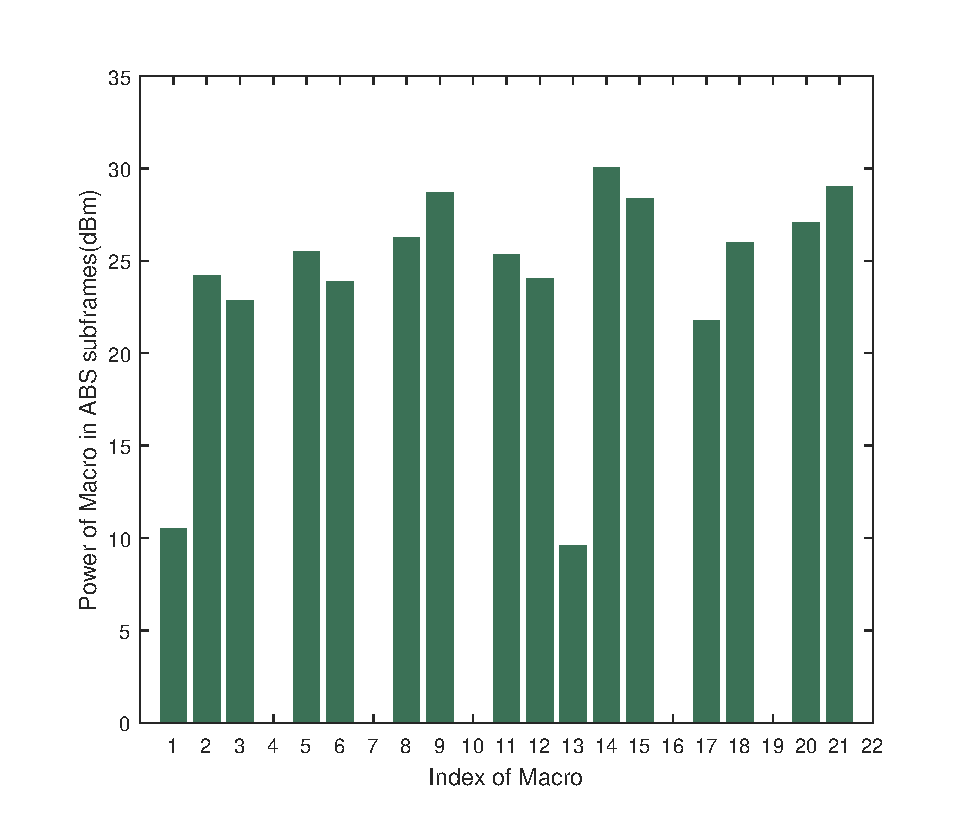
\includegraphics[width=.5\textwidth]{PowerOfMacro.eps}
\caption{Typical HetNet architecture with a macro cell and a pico cell, each cell regard as two logic cell.}
\label{F_PowerOfMacro}
\end{figure}

\begin{figure}[htpb]
\centering
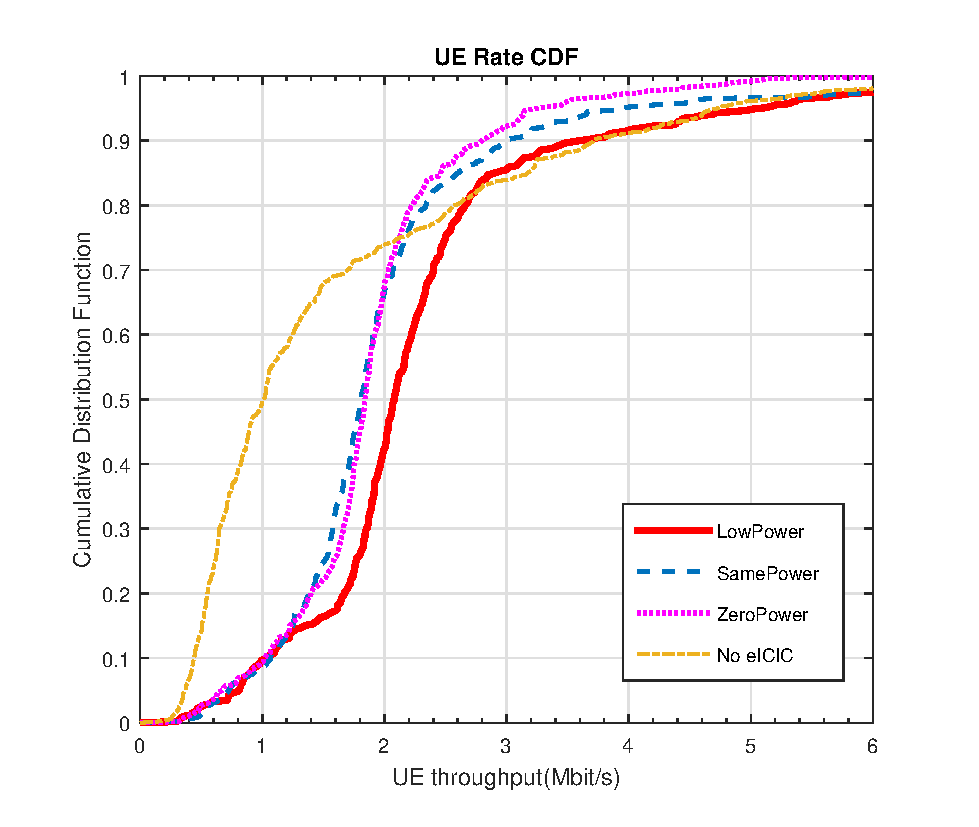
\includegraphics[width=.5\textwidth]{CumulativeDistributionFunction.eps}
\caption{The CDFs of global throughput.}
\label{F_ThroughputCDFs}
\end{figure}


\begin{figure}[htpb]
\centering
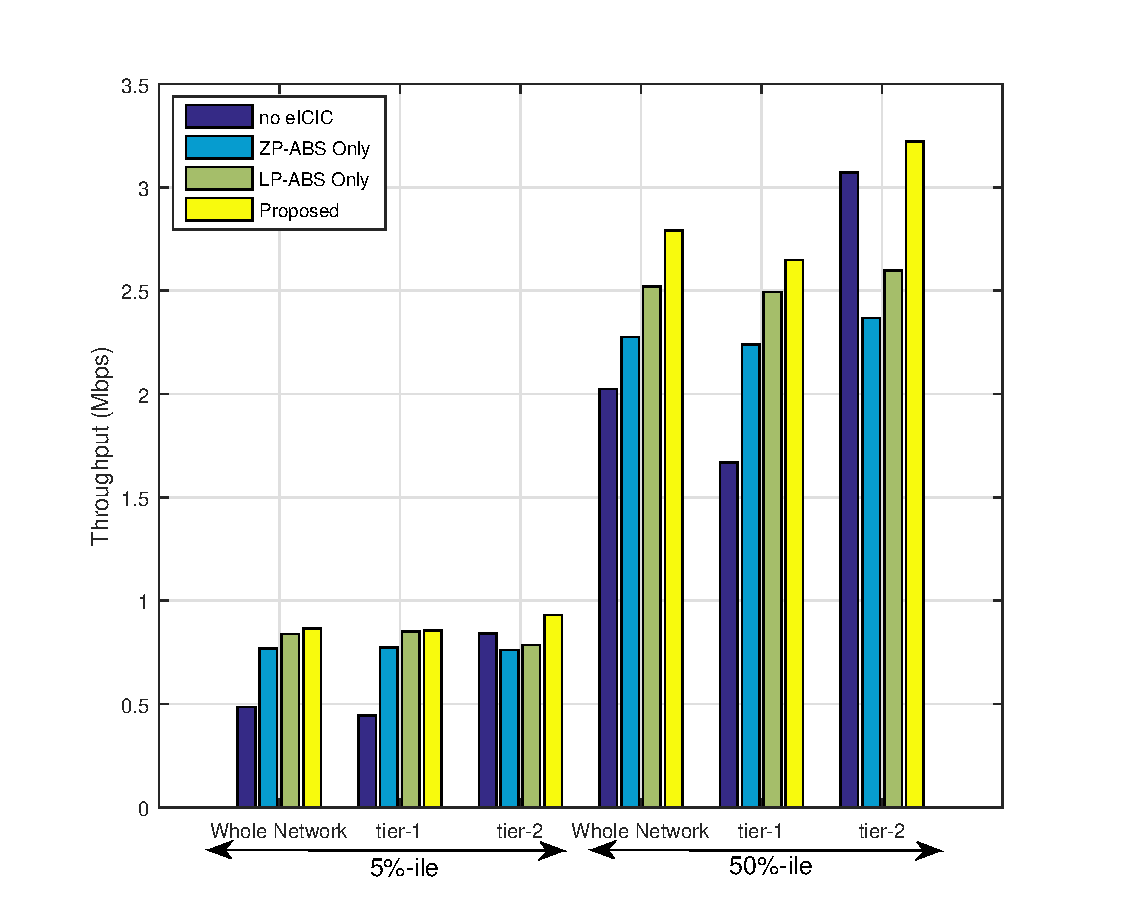
\includegraphics[width=.5\textwidth]{DetailedThroughputPerformance.eps}
\caption{Throughput performance with different scheme.}
\label{F_DetailedThroughput}
\end{figure}

Firstly, we discuss the power distribution of proposed scheme. From the Fig.\ref{F_PowerOfMacro} can be observed that five macro (4, 7, 10, 14, 15) transition power are almost zero which mean these macro cells are apply ZP-ABS. All these macro cells are included in seven macro cells which have picos, other two macro cells are apply LP-ABS with transition power for nearly 10dBm. The remaining macro station is applyed above 20dBm transmission power of LP-ABS. Such an arrangement can improve the overall throughput of the system, applying LP-ABS in a macro cells without picos, the interference suffered by victim pico UEs is mitigated and, at the same time, the performance of UEs in the macro cells with picos will not degrade much as the experienced SINR will not be significantly affected since they are assumed to use ZP-ABS.

Fig.\ref{F_ThroughputCDFs} shows the cumulative distribution function (CDF) of UE average throughput in the whole network which just show one of simulations. About 80\% of UEs access to a significantly improvement with our proposed algorithms against the other schemes.

In Fig.\ref{F_DetailedThroughput}, we plot the 5\%-ile and 50\%50-ile user throughput of the whole network, the tier-1 and tier-2 separately, and for both scenarios. We can observed the same trends for the 5\%-ile and 50\%50-ile user.
For no eICIC scheme. With our proposal, compared with the no eICIC in tier-1 58\% gain, compared with the ZP-ABS only and LP-ABS only in tier-2, there are respectively 27\% and 37\% of the gain. Thus, it includes both the gain of tier-1 being able to offload more users to the picos and protect the potential degradation in tier-2 from using LP-ABS. No eICIC scheme only guarantee tier-2 throughput because the user can not unload to pico in tier-1. Moreover, ZP-ABS only scheme can only guarantee tier-1 throughput, using the ZP-ABS in the tier-2 without picos can not maximize user throughput. For LP-ABS only scheme, since all macro use the same transition power in ABS subframes did not meet the non-uniform network topology.

Table \ref{T_Fairness} shows the fairness of throughput among UEs for different schemes. We consider the Jain's fairness index\cite{JainFairness} which can be expressed as $\frac{ (\sum_{u \in \mathcal{U}} R_u) }{ N \sum_{u \in \mathcal{U}} R_u^2}$, where $R_u$ is the throughput of UE-$u$, our proposed scheme increase 11\% than LP-ABS only and 40\% than no eICIC. Proprosed scheme and ZP-ABS can well guarantee fairness, proprosed scheme can improve total throughput at same time.

\begin{table}[!t]
\renewcommand{\arraystretch}{1.3}
\caption{Fairness for different schemes}\label{T_Fairness}
\centering
\begin{tabular}{c||c||c}
\hline
\bfseries Scheme & \bfseries Fairness index & \bfseries Total throughput\\
& &(Mbps)\\
\hline\hline\hline
no eICIC & 0.612 & 1239.2\\
ZP-ABS Only & 0.752 & 1266.9\\
LP-ABS Only & 0.688 & 1421.1\\
Proposed & 0.747 & 1528.5\\
\hline
\end{tabular}
\end{table}

%GATHER{reference.bib}
\section{Conclusion}\label{conclusion}
We consider an non-uniform HetNet topology where picos are deployed only in some macro cells. We consider using ZP-ABS and LP-ABS coordination among macro eNBs, ZP-ABS is applied only in same macros with deployed picos, while LP-ABS is using for other cells. We consider a joint problem of power and resource allocation. The goal is to maximize the PF utility, and solve this problem. The simulation results demonstrated that our proposed algorithms improve the user throughput in both the macros with picos and without picos.

\appendix[Step Size of Lagrangian dual decomposition]
The stepsize dynamically updates according to the rule
\begin{align}
\delta(t) = \gamma(t)\frac{D(\mu(t))-D(t)}{\| \partial D(\mu(t)) \|}, 0 < \underline{\gamma} \leq \gamma(t) \leq \overline{\gamma} < 2,
\end{align}
where $D(t)$ is an estimate of the optimal value $D^*$ of problem (\ref{dualProblem}), $\underline{\gamma}$ and $\overline{\gamma}$ are some scalars\cite{ConvexOptimization}. Consider a procedure for updating $D(t)$, where $D(t)$ is given by
\begin{align}
D(t) = \min_{0 \leq \tau \leq t} D(\mu (\tau)) - \varepsilon(t),
\end{align}
and $\varepsilon(t)$ is updated according to 
\begin{align}
\varepsilon(t+1)= 
&\left\{
\begin{matrix}
\rho \varepsilon(t),~~if D(\mu(t+1)) \leq D(\mu(t)), \\
\max\{  \beta \varepsilon(t), \varepsilon \}, otherwise,
\end{matrix}
\right.
\end{align}
where $\varepsilon$, $\beta$ and $\rho$ are fixed positive constants with  $\beta<1$
 and $\rho>1$\cite{ConvexOptimization}.
%GATHER{reference.bib}
\bibliographystyle{IEEEtran}
\bibliography{reference}
\end{document}
